\section{Auswertung}
\subsection{ Einleitung und Zielsetzung}
Die im Labor aufgenommenen Messwerte und die mithilfe des KiCads erstellten Simulationswerte werden in diesem Abschnitt für verschiedene Arten der Oszillatoren dargestellt. Durch den Vergleich der Messwerten sowie der Simulationsergebnissen mit der Theorie wird die Realisierung verschiedener Oszillatoren genauer untersucht.

\subsection{Der Phasenschieberoszillator}

Ein Phasenschieberoszillator besteht aus einem invertierenden Verstärker und einem rückgekoppelten passiven Hochpassfilter 3.Ordnung.

 \begin{figure}[H]
  \centering
  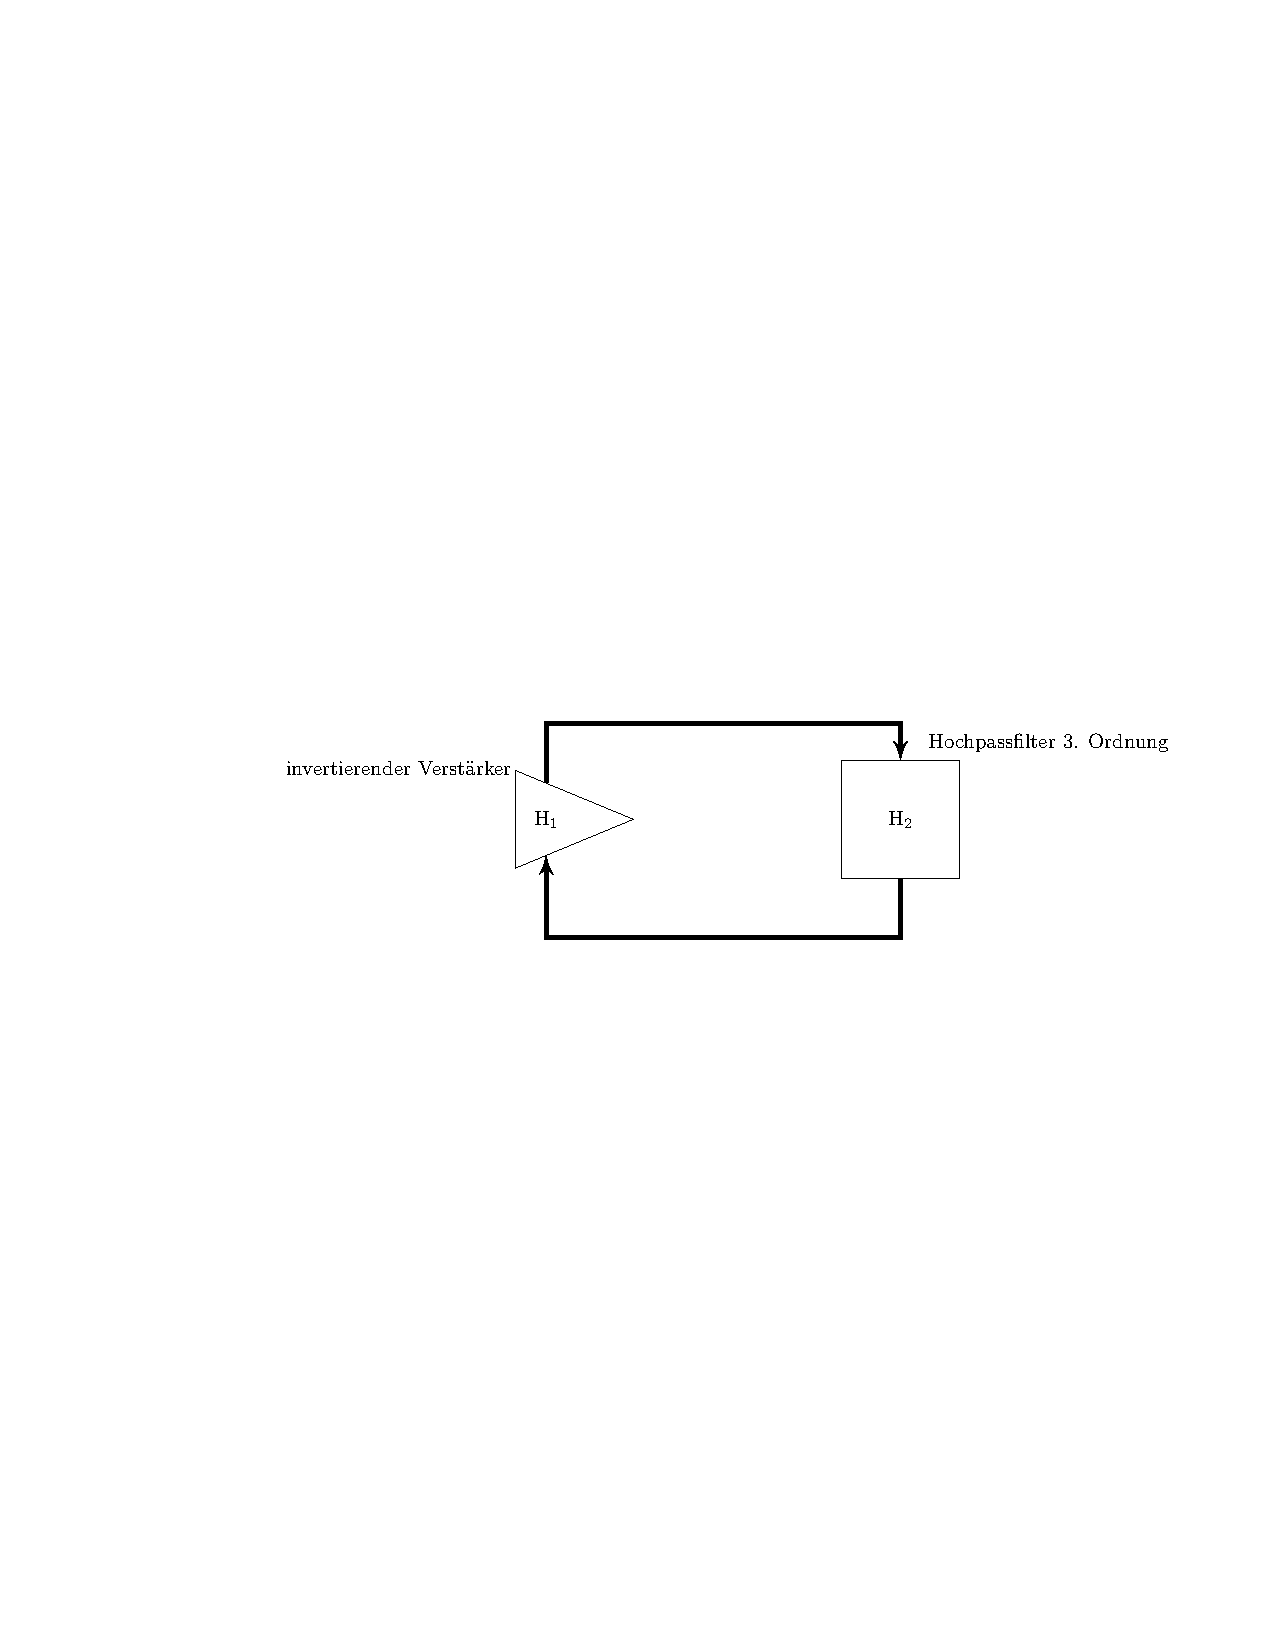
\includegraphics[width=\linewidth]{Elektronik-Laborprotokoll_Filter/Abbildungen/Blockschaltbild_Phasenschieberoszillator.pdf}
  \caption{Blockschaltbild: Phasenschieberoszillator}
  \label{fig:Phasenschieberoszillator_Block}
\end{figure}



Der Ausgang des invertierenden Verstärkers wird an den Eingang des Hochpassfilters 3. Ordnung und der Ausgang des Hochpassfilters an den Eingang des invertierenden Verstärkers angeschlossen.

Damit die Schaltung oszilliert, muss für den Betrag der Schleifenverstärkung des Systems die folgenden Bedingungen \cite{Skript} gelten:

\begin{equation}
|V| \cdot |K| \geq 1
\end{equation}

\begin{equation}
\label{eq:Phase_Formel}
(\phi_V + \phi_K) = n \cdot 360^\circ
\end{equation}
Das heißt, dass das Produkt aus den Beträgen der Amplitudenverstärkung von dem invertierenden Verstärker und dem Hochpassfilter mindestens so groß wie 1 sein soll. Zusätzlich sollte die Summe der Phasenverschiebungen ein Vielfaches von \SI{360}{\degree} sein.

Wie es in der Theorie \ref{eq:invertierender_Verstärker_180_degree} ausführlich erklärt wurde, beträgt die Phasenverschiebung eines invertierenden Verstärkers \SI{180}{\degree}. Aus der Formel \ref{eq:Phase_Formel} folgt:

\begin{equation*}
 \phi_K = 360^\circ - \phi_V = 360^\circ -(180^\circ)=180^\circ
\end{equation*}

Eine Phasendrehung von \SI{0}{\degree} bis \SI{270}{\degree} kann man mithilfe eines Hochpassfilters 3.Ordnung erreichen . Das heißt, es existiert dabei schon eine Frequenz, wobei die Phasendrehung \SI{180}{\degree} beträgt. 

Das Ziel war, ein Phasenschieberoszillator mit einer Oszillationsfrequenz von \SI{1}{\kilo\hertz} zu entwerfen. Das heißt, erstens soll ein passiver Hochpassfilter 3.Ordnung so dimensioniert werden, dass bei einer Frequenz von \SI{1}{\kilo\hertz} eine Phasendrehung von \SI{180}{\degree} erreicht wird.

In die Übertragungsfunktion eines Hochpassfilters dritter Ordnung (siehe \ref{subsec:Hochpass_3}), setzt  man die Kreisfrequenz \(\omega\) ein, bei der der Phasenwinkel von \(H(s)\) etwa 180 Grad beträgt.

Die Frequenz \(\omega\) in $rad/s$ für 1000 Hz ist:
\begin{equation}
\omega = 2 \pi f = 2 \pi \times 1000 \, \text{Hz} \approx 6283.19 \, \text{rad/s}
\end{equation}

Durch numerische Iteration über verschiedene \(\tau\) Werte lässt sich ermitteln, dass bei \(\tau \approx 6.54 \times 10^{-5}\) Sekunden der Phasenwinkel des Filters \SI{180}{\degree}  bei dieser Frequenz erreicht.

Da \(\tau = RC\), und \(C\) ist gegeben als \SI{100}{\nano\farad} lässt sich der Wert des Widerstands \(R\) wie folgt berechnen:
\begin{align}
C &= 100 \, \text{nF} = 100 \times 10^{-9} \, \text{F} \\
\tau &= RC \\
R &= \frac{\tau}{C} = \frac{6.54 \times 10^{-5}}{100 \times 10^{-9}} \, \Omega \\
R &\approx 654 \, \Omega
\end{align}

Jetzt kann man berechnen, wie groß die Amplitudenverstärkung des Hochpassfiltes bei der Oszillatonsfrequenz von \SI{1000}{\hertz} ist, wenn man die berechneten und die gegebenen Werte in die Übertragungsfunktion \ref{subsec:Hochpass_3} einsetzt:


Für die Amplitude bei einer Frequenz von \SI{1000}{\hertz} wird  \(s = j2\pi f\) gesetzt:
\begin{align*}
    H(j2\pi f) &= \frac{-6.94 \times 10^{-11} \cdot j \cdot f^3}{-6.94 \times 10^{-11} \cdot j \cdot f^3 - 1.01 \times 10^{-6} \cdot f^2 + 0.00205 \cdot j \cdot f + 1.0} \\
    H(j2\pi \cdot \SI{1000}{\hertz}) &= -0.0350 + 0.000231 \cdot j \\
    |(H(j2\pi \cdot \SI{1000}{\hertz}))| &= \frac{1}{28,6}
\end{align*}

Da $|K| = \frac{1}{28.6}$ ist, folgt aus der Gleichung  $ |V| \cdot |K| \geq 1 $ :

\begin{equation*}
     |V| \geq 28,6
\end{equation*}

Die Verstärkung des Operationsverstärkers (Op-Amp) sollte mindestens 28,6 betragen. Die Verstärkung eines invertierenden Verstärkers ist gegeben durch:
\begin{align*}
    V &= \frac{R4}{R5}
\end{align*}
Daraus folgt, dass das Verhältnis \( \frac{R4}{R5} \) mindestens 28,6 sein muss.

Im Labor wurde anstelle der genauen berechneten Werte der Widerstände (\SI{654}{\ohm}) des Hochpassfilters, den nahsten Widerstand  (\SI{680}{\ohm}) benutzt, so dass
$R_1=R_2=R_3=680$ war. 

Die Oszillation war durch eine Verstärkung von 28,6 des invertierenden Verstärkers theoretisch möglich. Jedoch wurde die aufgebaute Schaltung unter Berücksichtigung der Leistungverluste wegen der realen Bauelemente so dimensioniert, dass die theoretische Verstärkung deutlich größer ist, als die notwendige.

 $R_4=(\SI{56}{\kilo\ohm}$ und $R_5=\SI{120}{\kilo\ohm}$ wurde benutzt, sodass \[ \frac{R_4}{R_5} = \frac{56000}{120} = 466.6 \geq 29\] 

In der Abbildung \ref{fig:hochpass3ordnungbode} ist das Bode-Diagram des Hochpassses 3.Ordnung  dargestellt.


\begin{figure}[H]
  \centering
  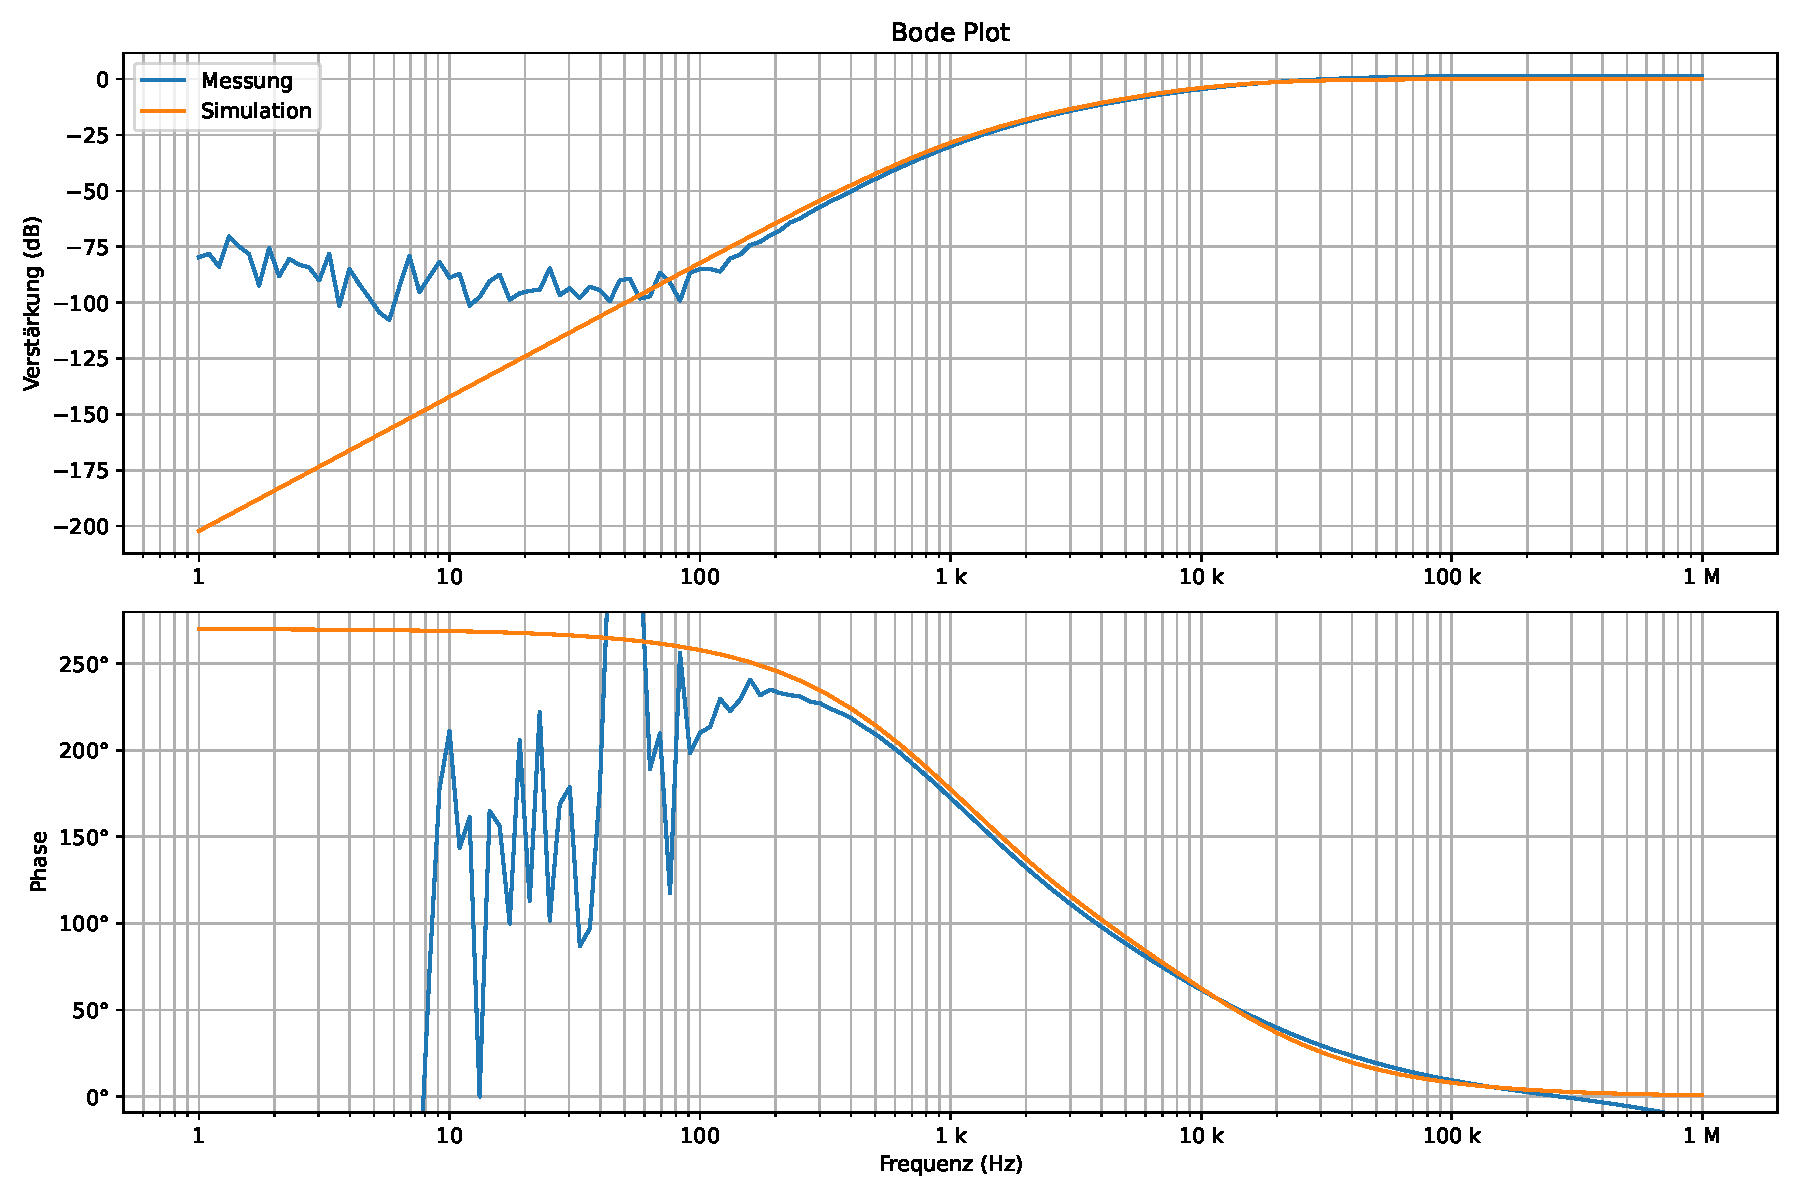
\includegraphics[width=\linewidth]{Elektronik-Laborprotokoll_Filter/Plots/hochpass3ordnungbode.pdf}
  \caption{Bode-Diagramm des Hochpasses 3. Ordnung}
  \label{fig:hochpass3ordnungbode}
\end{figure}

%Erstens Plots zu den Aufgaben zuordnen
In der Betrachtung eines Bode-Diagramms eines Hochpasses dritter Ordnung \ref{fig:hochpass3ordnungbode} liegt die Grenzfrequenz bei etwa \SI{12}{\kilo\hertz}. Die Phasenverschiebung erstreckt sich von \ang{270} bis \ang{0}.Bei niedrigeren Frequenzen wird zudem ein stärkerer Einfluss des Rauschens auf das Diagramm deutlich, was zu einer sehr unregelmäßigen Phasenberechnung in diesem Bereich führt. Es fällt auf, dass bei einer Frequenz von \SI{955}{\hertz} die Phasenverschiebung beinahe \ang{180} erreicht. \\
Das Ziel war eigentlich, eine Phasendrehung von \SI{180}{\degree} bei der gewünschten Oszillatonsfrequenz bzw. bei \SI{1}{\kilo\hertz} zu erreichen. Die Abweichung liegt daran, dass auch in der Simulation die Schaltung mit den Widerstandswerten, die nah an den berechneten Werten stehen, aber im Labor zu finden waren, dimensioniert wurde.

Ein weiteres bemerkenswertes Merkmal zeigt sich darin, dass die Amplitude bei ungefähr \SI{1}{\kilo\hertz} bei \SI{-29}{\decibel} liegt, was in etwa dem Wert \(\frac{1}{29}\) entspricht.
%Es gibt das Gefühl, dass der TExt oben von Chatgpt geschrieben wurde. Mach mal KI Prüfung :) Oder hat man Deutsch C3 ..alles gut

%Kein Pronomen benutzen, kein wir kein ich
%"Daraus wird es herauskristallisiert" sowas möchte ich gerne benutzen %Ich denke Phasenschieber-OSzi-Diagramm 3 ist zu viel.  1-2 reichen aus. Oder lass ich so erstmal
%#original: Wir können ein Bodeplot dritte ordnung hochpass beobachten, die Grenzfrequenz ist ungefähr 12k Ohm, Phaseversschibung geht von 270 bis 0, und wir können sehen dass bei 955 ist es fast 180, wir können auch klar beobachten, dass bei kleinere frequenzen hat der Geräusch eine großere einfluss auf das Diagram, und auf diesen Gründ verhält sich die Phase berechnung sehr Chaotisch bei niedrige frequenzen.
%Hier Beschreibung Auswertung Bode, Phasendrehung erwähnen, Dämpfung erwähnen, hauptsächlich bei 1kHz eine Dämpfung von -29db entsprich t 1/29 ungefähr...
%Das kommt am erestens, Bode Diagram :p Bode ist oben
In der Abbildung \ref{fig:phasenschieberozillator1} ist die Spannung am Ausgang des simulierten Phanschieberoszillators für einen langen Zeitabschnitt dargestellt.

\begin{figure}[H]
  \centering
  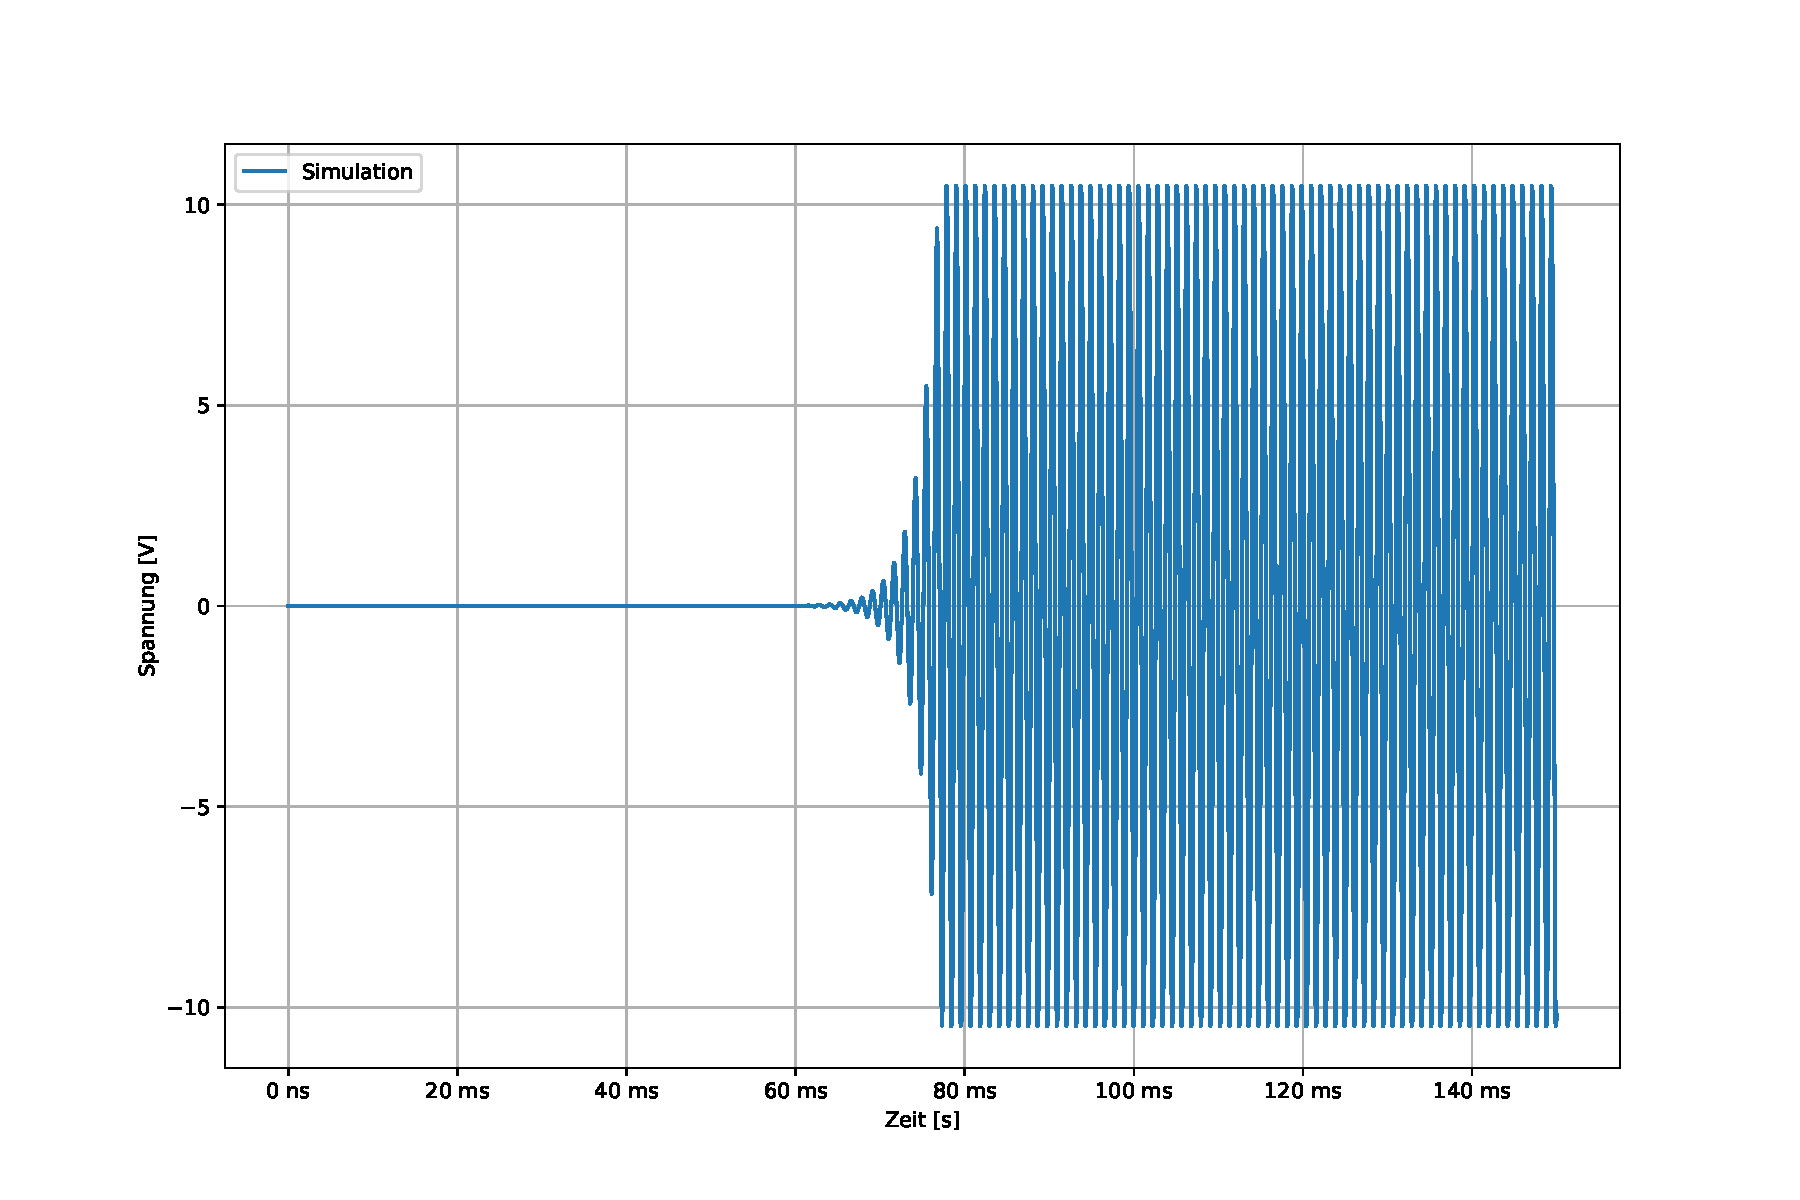
\includegraphics[width=\linewidth]{Elektronik-Laborprotokoll_Filter/Plots/phasenschieberozillator1.pdf}
  \caption{Phasenschieber-Oszillator-Diagramm 1}
  \label{fig:phasenschieberozillator1}
\end{figure}

 In dieser Darstellung \ref{fig:phasenschieberozillator1} wird eine Simulation des Phasenschieber-Oszillators gezeigt. Man kann beobachten, dass das Signal zwischen 0 und 60 ms zu schwach ist, um es deutlich zu erkennen. Allerdings wird das exponentielle Wachstum der Signalgröße ab 80 ms sichtbar. Der Operationsverstärker (\textit{Opamp}) ist zu diesem Zeitpunkt gesättigt, und das Signal bleibt konstant bei \SI{-12}{\volt} bis \SI{12}{\volt}. 


In der Abbildung \ref{fig:phasenschieberozillator2} ist die Spannung am Ausgang des simulierten Phanschieberoszillators für einen kürzeren Zeitabschnitt zusammen mit den Messwerten dargestellt.


\begin{figure}[H]
  \centering
  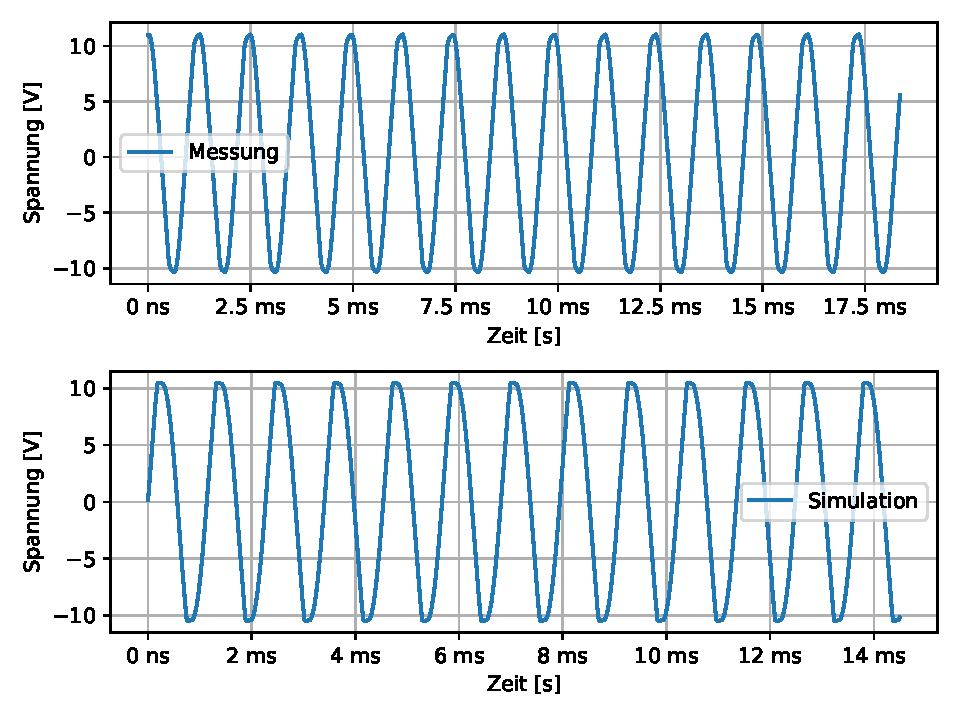
\includegraphics[width=\linewidth]{Elektronik-Laborprotokoll_Filter/Plots/phasenschieberozillator2.pdf}
  \caption{Phasenschieber-Oszillator-Diagramm 2}
  \label{fig:phasenschieberozillator2}
\end{figure}


In der Abbildung \ref{fig:phasenschieberozillator3} sind drei Perioden der Spannung jeweils am Ausgang des simulierten und aufgebauten Phanschieberoszillators dargestellt.


\begin{figure}[H]
  \centering
  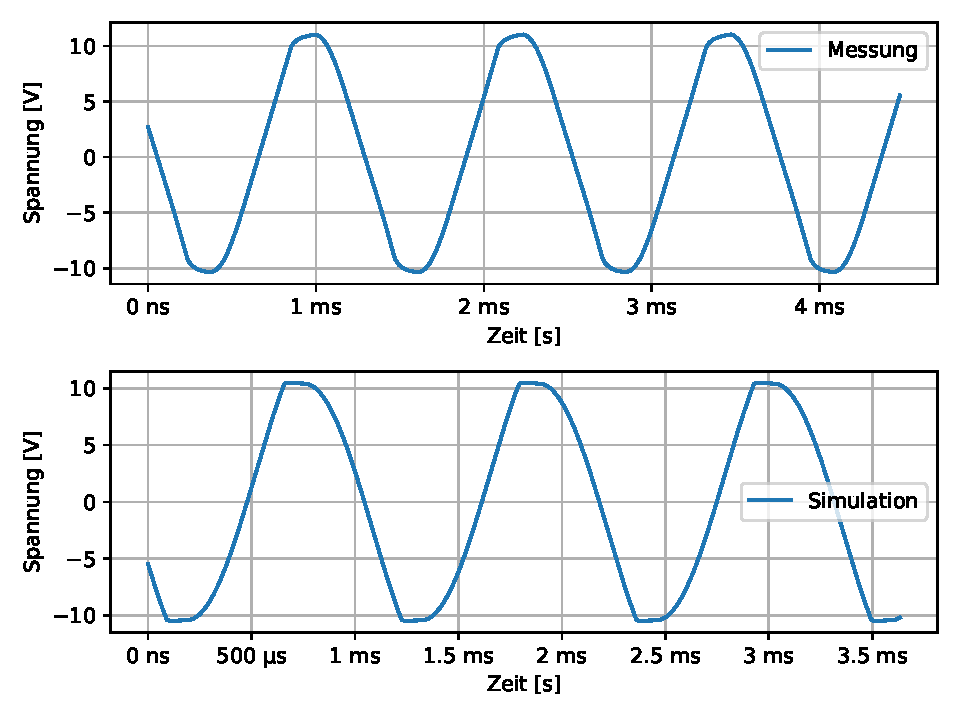
\includegraphics[width=\linewidth]{Elektronik-Laborprotokoll_Filter/Plots/phasenschieberozillator3.pdf}
  \caption{Phasenschieber-Oszillator-Diagramm 3}
  \label{fig:phasenschieberozillator3}
\end{figure}

Die Darstellung einer geringeren Anzahl der Perioden der Spannung am Ausgang des Phasenschieber-Oszillators ermöglicht, die tatsächliche Frequenz davon genauer zu bestimmen.\\
Sowohl die Frequenz des simulierten als auch aufgebauten Oszillators beträgt zwischen \SI{800}{\hertz} und  \SI{900}{\hertz}. Während die Abweichung der Messung von der Simulation an Messungenauigkeiten liegen kann, liegt die Abweichung der Simulation von der Theorie daran, dass auch bei der Simulation die Schaltung nicht mit den genau berechneten Werten sondern mit den Werten der tatsächlich verwendeten Bauteile dimensioniert wurde.

\subsection{NE555}
%NE555 beschreiben, was es macht
Als einer der weltweit bekanntesten ICs findet der NE555 Anwendung in verschiedenen Elektronikschaltungen. In diesem Teilversuch werden verschiedene Konfigurationen von NE555, wie der Schmitt-Trigger und der Monoflop, genauer untersucht.
\subsubsection{Astabile Kippstufe}

In diesem Teilversuch wurde der NE555 zunächst als Schmitt-Trigger eingesetzt. Aufgrund der invertierenden Eigenschaften des Schmitt-Triggers sind der Ausgang und Eingang der Schaltung komplementär zueinander, wodurch $C_1$ kontinuierlich über $R_1$ auf- und entladen wird. Das Ziel war, erstens eine astabile Kippstufe mit einem Tastgrad von \SI{50}{\percent} zu dimensionieren.

Wenn die Spannung am Kondensator bis auf $1/3 V_{CC}$ sinkt, beginnt der Ladevorgang. Wenn die Spannung am Kondensator bis auf $2/3 V_{CC}$ steigt \cite{tietze1991electronic}, beginnt der Entladevorgang. Für einen Tastgrad von \SI{50}{\percent} gilt:

\begin{equation*}
    t_{Lade} =t_{Entlade}
\end{equation*}

Der Entladevorgang eines Kondensators gilt die folgende Gleichung:
\begin{equation}
    U_C(t)=U_0 \cdot (1-e^{\frac{-t}{\tau}})
\end{equation}
%
\begin{align*}
    U_C(t_{entlade})=U_0 \cdot (1-e^{\frac{-t_{entlade}}{\tau}})
\end{align*}
%
\begin{align*}
   \frac{1}{3}V_{CC}=  \frac{2}{3}V_{CC} \cdot (1-e^{\frac{-t_{entlade}}{\tau}})
\end{align*}
%
\begin{align*}
   \frac{1}{2} =  (1-e^{\frac{-t_{entlade}}{\tau}})
\end{align*}
%
\begin{align*}
   \frac{1}{2}  = e^{\frac{-t_{entlade}}{\tau}}
\end{align*}
%
\begin{align*}
   ln(2)  = \frac{t_{entlade}}{\tau}
\end{align*}
Durch die Gleichung $\tau=R_1C$ folgt:
\begin{align*}
   ln(2)  = \frac{t_{entlade}}{RC_1}
\end{align*}
Durch die Umformung folgt:
\begin{align*}
  R  = \frac{t_{entlade}}{ln(2)C_1}
\end{align*}
%
Da der Tastgrad \SI{50}{\percent} ist, gilt: $t_{entlade}= \frac{1}{2}T $. Darus folgt:
\begin{align*}
  R  = \frac{T}{2ln(2)C_1}
\end{align*}
Durch die Gleichung $f=\frac{1}{t}$ folgt:
\begin{align*}
  R  = \frac{1}{2ln(2)\cdot fC_1}
\end{align*}
Durch die Einsetzung der gegebenen Werte für $f$ und $C$  folgt:
\begin{align*}
  R  = \frac{1}{2ln(2)\cdot \SI{10}{\kilo\hertz}\cdot \SI{100}{\nano\farad}}=\SI{721,35}{\ohm}
\end{align*}
%
Der ideale Widerstand, um die gewünschten Voraussetzungen zu erfüllen, wäre zwar \SI{721,35}{\ohm} gewesen, jedoch wurde aufgrund der begrenzten verfügbaren Widerstandswerte im Labor der nächstgelegene Widerstand von \SI{680}{\ohm} verwendet.

In der Abbildung \ref{fig:oszillator} ist die astabile Kipsstupe mit einer Oszillationsfrequenz von \SI{10}{\kilo\hertz} und einem Tastgrad von \SI{50}{\percent} dargstellt.
\begin{figure}[H]
  \centering
  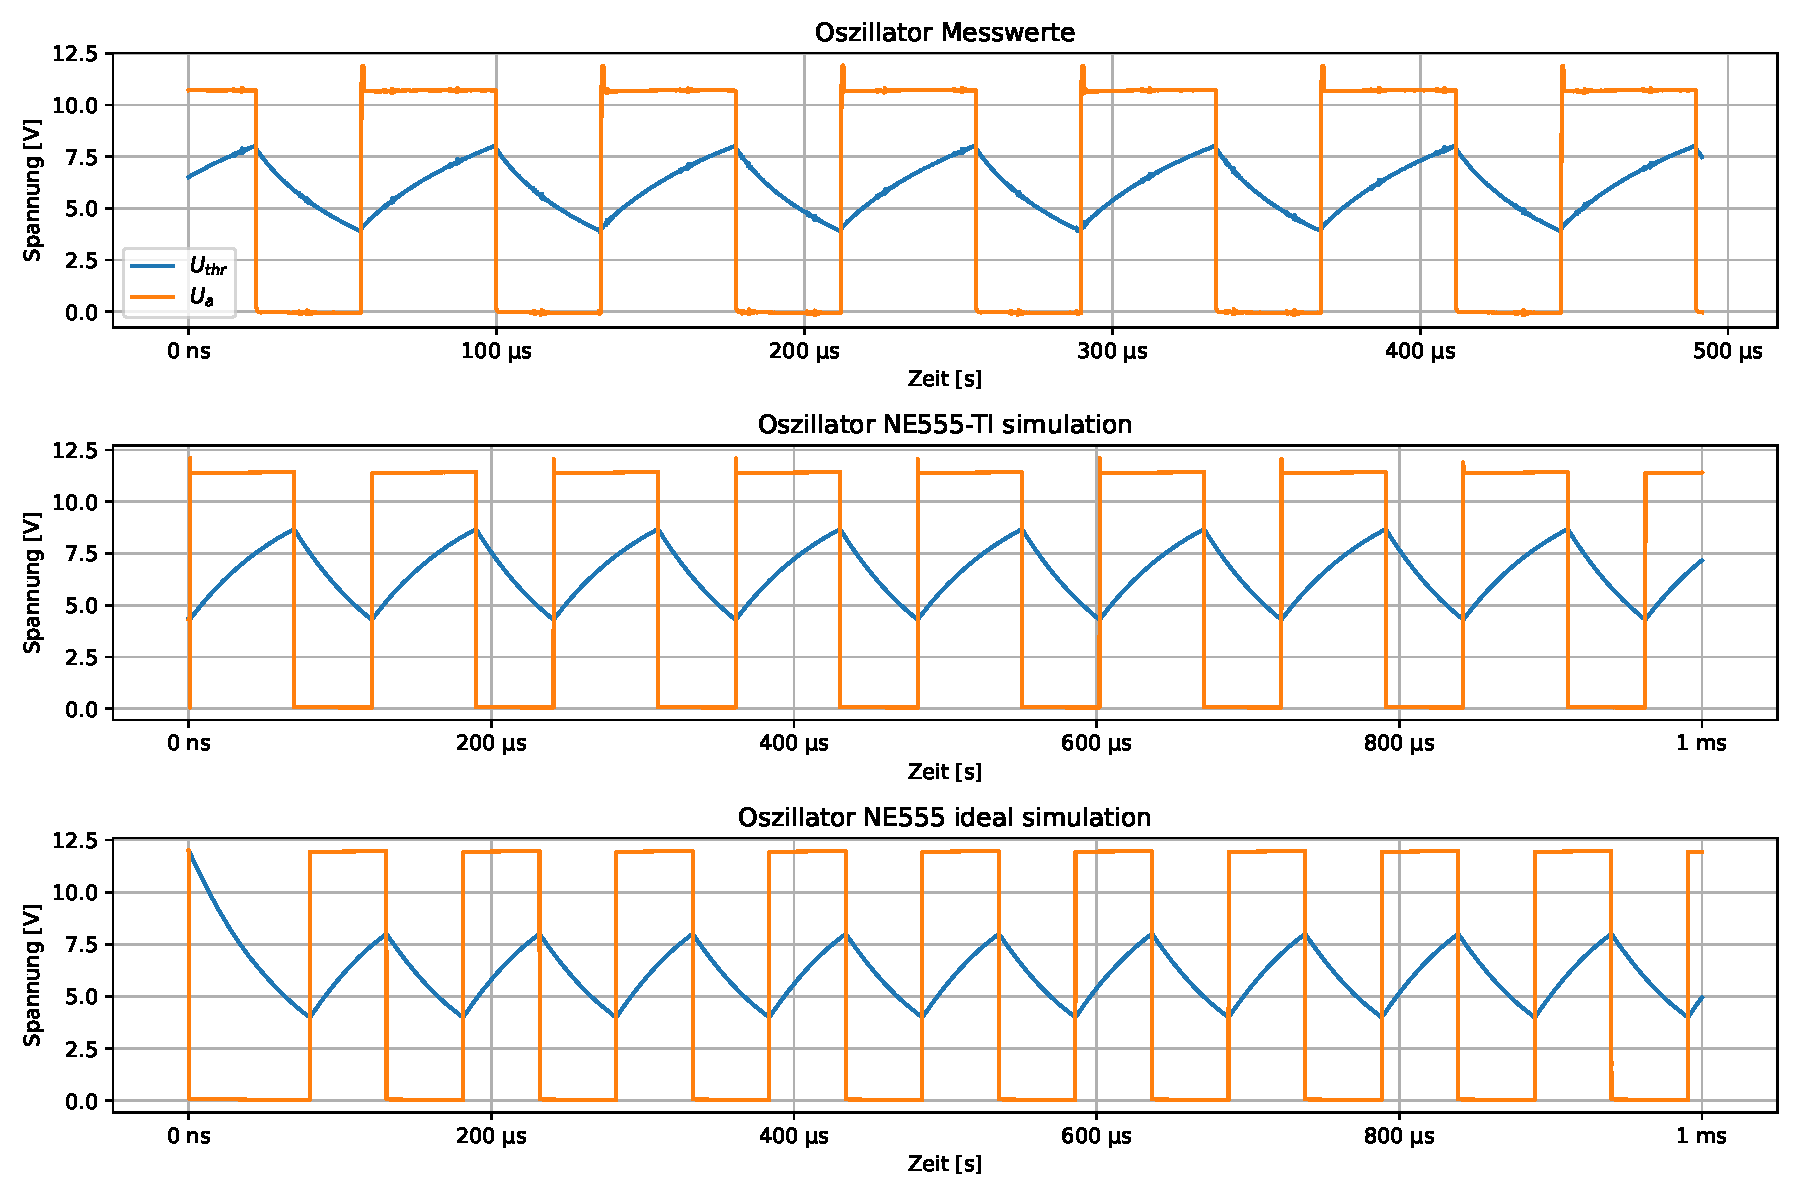
\includegraphics[width=\textwidth]{Elektronik-Laborprotokoll_Filter/Plots/oszillator.pdf}
  \caption{Oszillator-Diagramme}
  \label{fig:oszillator}
\end{figure}
Drei Diagramme werden betrachtet in \ref{fig:oszillator}: Messwerte, eine Simulation, die die interne Schaltung des NE555 berücksichtigt, und eine ideale Simulation, die von einer idealisierten NE555 ausgeht. Auffällig ist, dass die ersten beiden Diagramme einander sehr ähnlich sind und sogar gemeinsame Merkmale aufweisen. Beispielsweise steigt die Spannung zunächst auf etwa 12V, fällt dann aber in kurzer Zeit auf 10V und bleibt auf diesem Niveau. Im Gegensatz dazu zeigt die idealisierte Simulation eine kontinuierliche Schwingung zwischen 12V und 0V ohne Überschwingen. Die TI-Simulation wurde mit KiCad erstellt, während die idealisierte Simulation mittels LTSpice durchgeführt wurde. Deutlich sichtbar ist die Aufladungs- und Entladungskurve des Kondensators, wobei $U_{thr}$ die Spannung am Schwellenwert und $U_{a}$ die Ausgangsspannung, wie in anderen Schaltungen auch, darstellt.

Bei den aufgebauten Schaltung erreicht die Spannung nicht den maximalen Wert der Versorgungsspannung, obwohl dies bei der idealen Simulation der Fall ist.
Der gemessene Tastgrad, basierend auf den Messwerten und den Simulationsergebnissen, die tatsächlich die interne Schaltung des NE555 berücksichtigen, beträgt etwa \SI{58}{\percent}. Dieser Wert weicht sowohl von der idealisierten Simulation als auch vom theoretisch erwarteten Tastgrad von \SI{50}{\percent} ab. Obwohl Messungenauigkeiten zu dieser Abweichung beitragen können, liegt der Hauptgrund in der internen Schaltung von NE555.\\

Durch die Auswahl des Widerstandswerts ist es möglich, den Tastgrad nach Belieben einzustellen. Unten sind Beispiele für einen Tastgrad von \SI{25}{\percent} und \SI{75}{\percent} aufgeführt. Die Abweichungen der Messwerte sind hauptsächlich auf die interne Schaltung des NE555 zurückzuführen

%
Dargestellt ist in der Abbildung \ref{fig:einstellbaretastgrad25} der Verlauf der Ausgangsspannung und der Spannnung am Kondensator bei einem Tastgrad von \SI{25}{\percent}.
%
\begin{figure}[H]
  \centering
  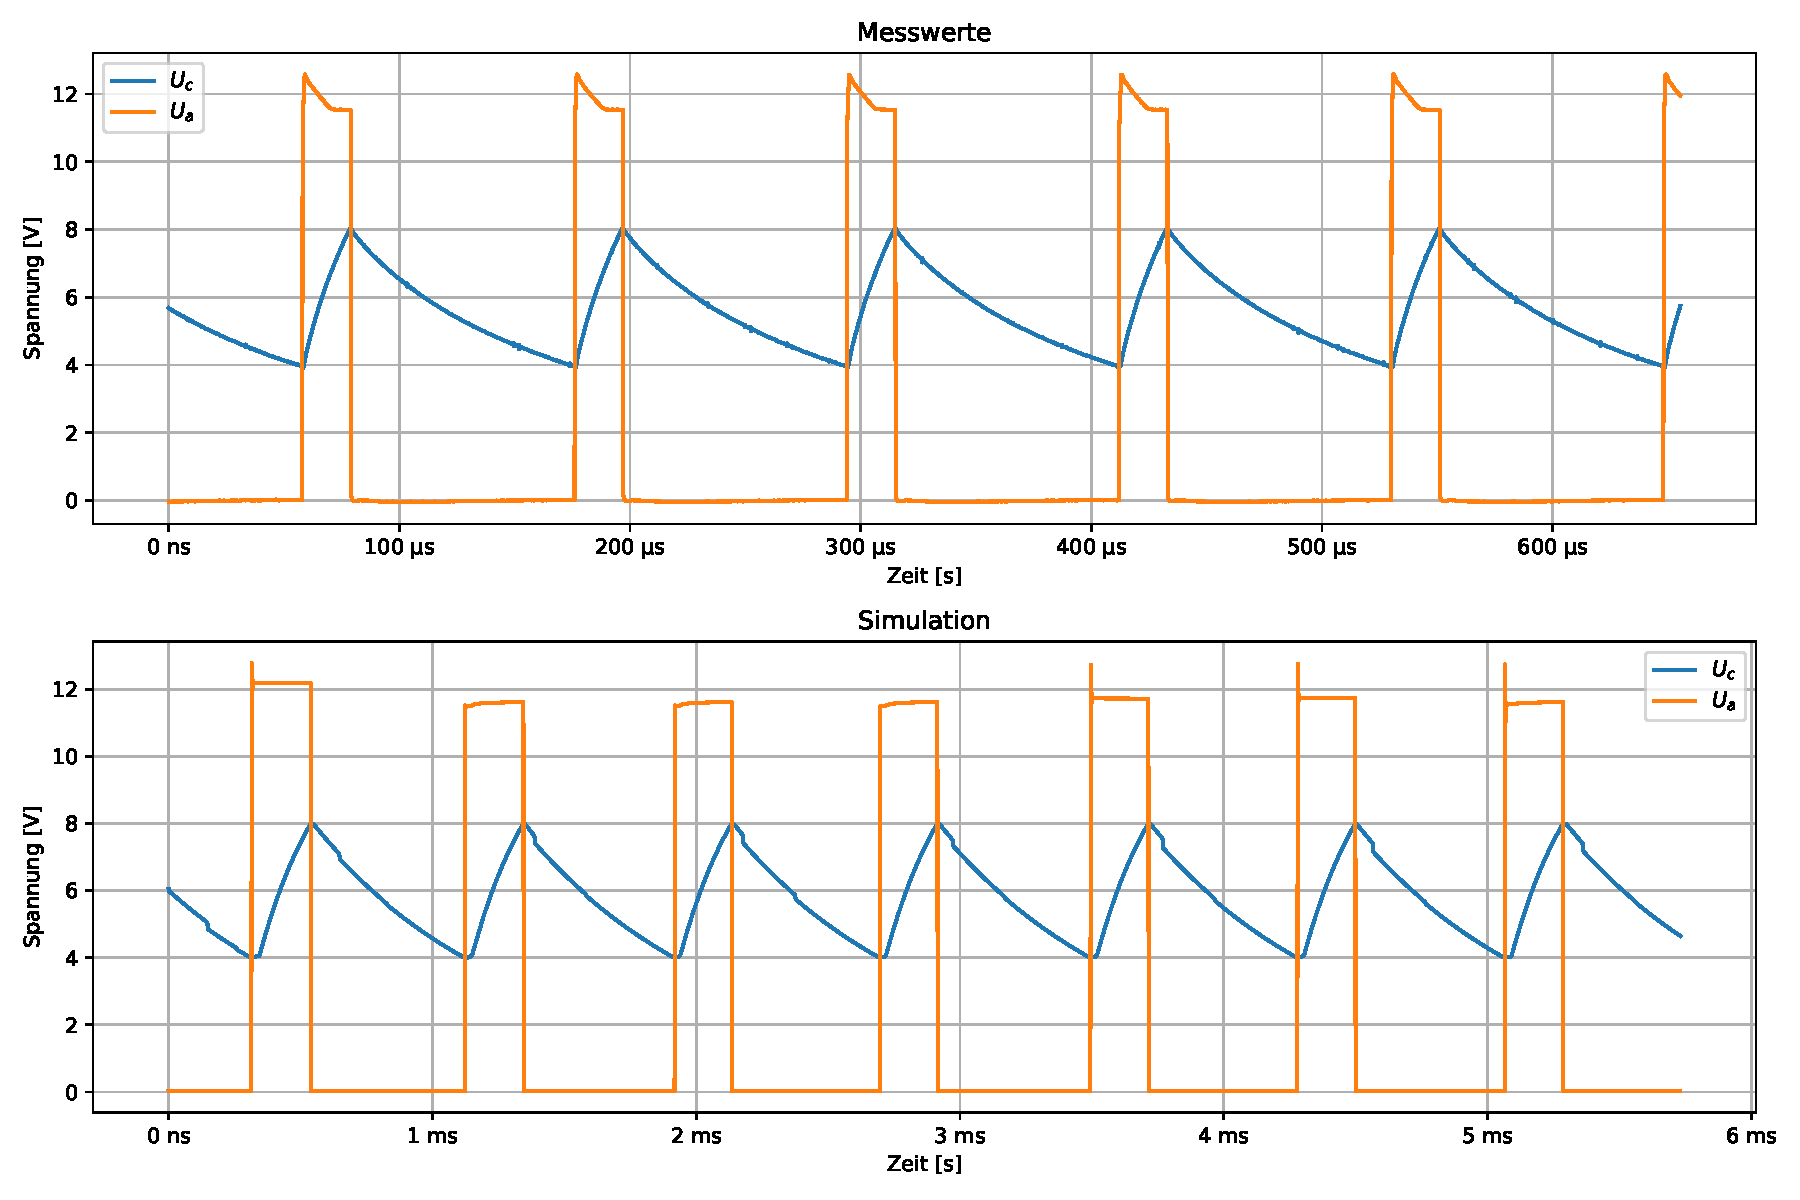
\includegraphics[width=\linewidth]{Elektronik-Laborprotokoll_Filter/Plots/einstellbaretastgrad25.pdf}
  \caption{Einstellbarer Tastgrad-Diagramm (25\%)}
  \label{fig:einstellbaretastgrad25}
\end{figure}



%
Dargestellt ist in der Abbildung \ref{fig:einstellbaretastgrad75} der Verlauf der Ausgangsspannung und der Spannnung am Kondensator bei einem Tastgrad von \SI{75}{\percent}.
\begin{figure}[H]
  \centering
  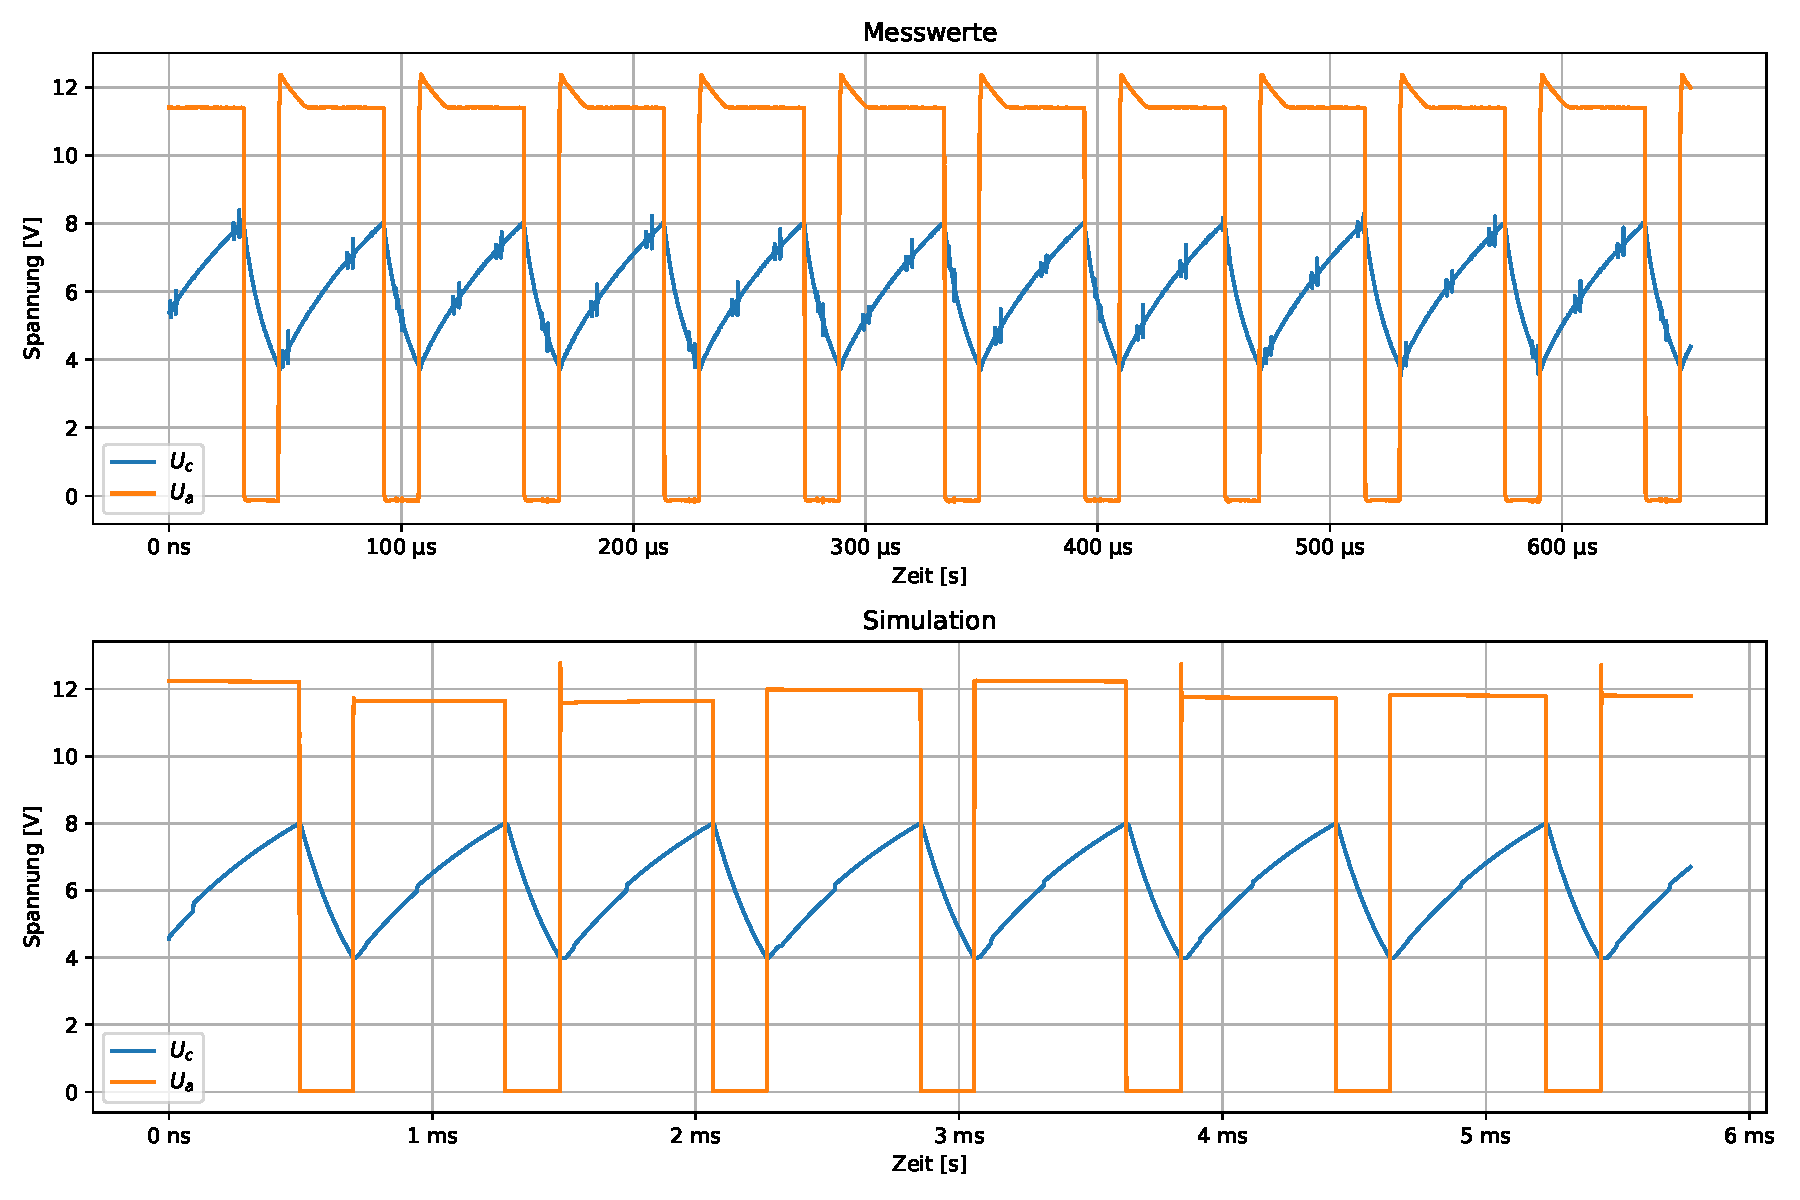
\includegraphics[width=\linewidth]{Elektronik-Laborprotokoll_Filter/Plots/einstellbaretastgrad75.pdf}
  \caption{Einstellbares Tastgrad-Diagramm (75\%)}
  \label{fig:einstellbaretastgrad75}
\end{figure}

%(?)WOhin der Abschnitt gehört
In den Abbildungen \ref{fig:einstellbaretastgrad75} lässt sich der Zusammenhang zwischen der Kondensatorspannung und der erzeugten Schwingung sehr gut erkennen. Zuerst wird der Kondensator über den Widerstand aufgeladen, bis die Spannung am Kondensator 8 V (2/3 der VCC) erreicht. Anschließend schaltet der erste Schmitt-Trigger (THR) um, und der Ausgang wird auf LOW gesetzt. Danach erfolgt die Entladung des Kondensators, und die Spannung am 2. Pin (TRI) sinkt, bis sie 4 V (1/3 der VCC) erreicht. Hierbei tritt ein weiterer Schmitt-Trigger-Komparator in Aktion, und der Ausgang wird auf HIGH gesetzt. Damit schließt sich ein Zyklus ab und wiederholt sich erneut, wodurch die Oszillation erzeugt wird.

Die Schaltung ist nun mit unterschiedlichen Duty Cycles konfiguriert, wodurch sich der Kondensator über einen größeren Widerstand langsamer auflädt und entlädt. In Abbildung\ref{fig:einstellbaretastgrad75}  ist ein Duty Cycle von 75\% eingestellt. Es wird deutlich, dass das Aufladen länger dauert, da der Ladestrom durch einen größeren Widerstand fließt.
%
\subsubsection{Monoflop}
%
In diesem Teilversuch wird der NE555 im monostbilen Betriebsmodus verwendet. In diesem Modus geht der Schaltkreis nach einer Anregung für eine festgelegte Zeitspanne in den instabilen Zustand über, um dann wieder in den stabilen Zustand umzuschalten und dort bis zur nächsten Anregung zu verbleiben.\\
Das Ziel war einen Monoflop mit einer Zeitkonstante von $\tau=\SI{100}{\micro\second}$ aufzubauen.
Die Zeitkonstante ist wie folgt definiert:
\begin{equation}
    \tau=R\cdot C
\end{equation}
Im ganzen Versuch wurde ein Kondensator mit einer Kapazität von $C=\SI{100}{\nano\farad}$ verwendet. Die Gleichung für die Zeitkonstante kann man nach R umformen.
\begin{equation*}
R=\frac{\tau}{C}
\end{equation*}
Die gegebenen Werte für den Kondensator und die Zeitkonstante können in die Gleichung eingesetzt werden, um den Wert des Widerstands zu berechnen. Auf diese Weise kann die Dimensionierung der Schaltung abgeschlossen werden
\begin{equation*}
R=\frac{\SI{100}{\micro\second}}{\SI{100}{\nano\farad}}=\SI{1}{\kilo\ohm}
\end{equation*}
%
Die Abbildung \ref{fig:monoflop} zeigt den Spannungsverlauf am Trigger-PIN und am Ausgang der Schaltung.
\begin{figure}[H]
  \centering
  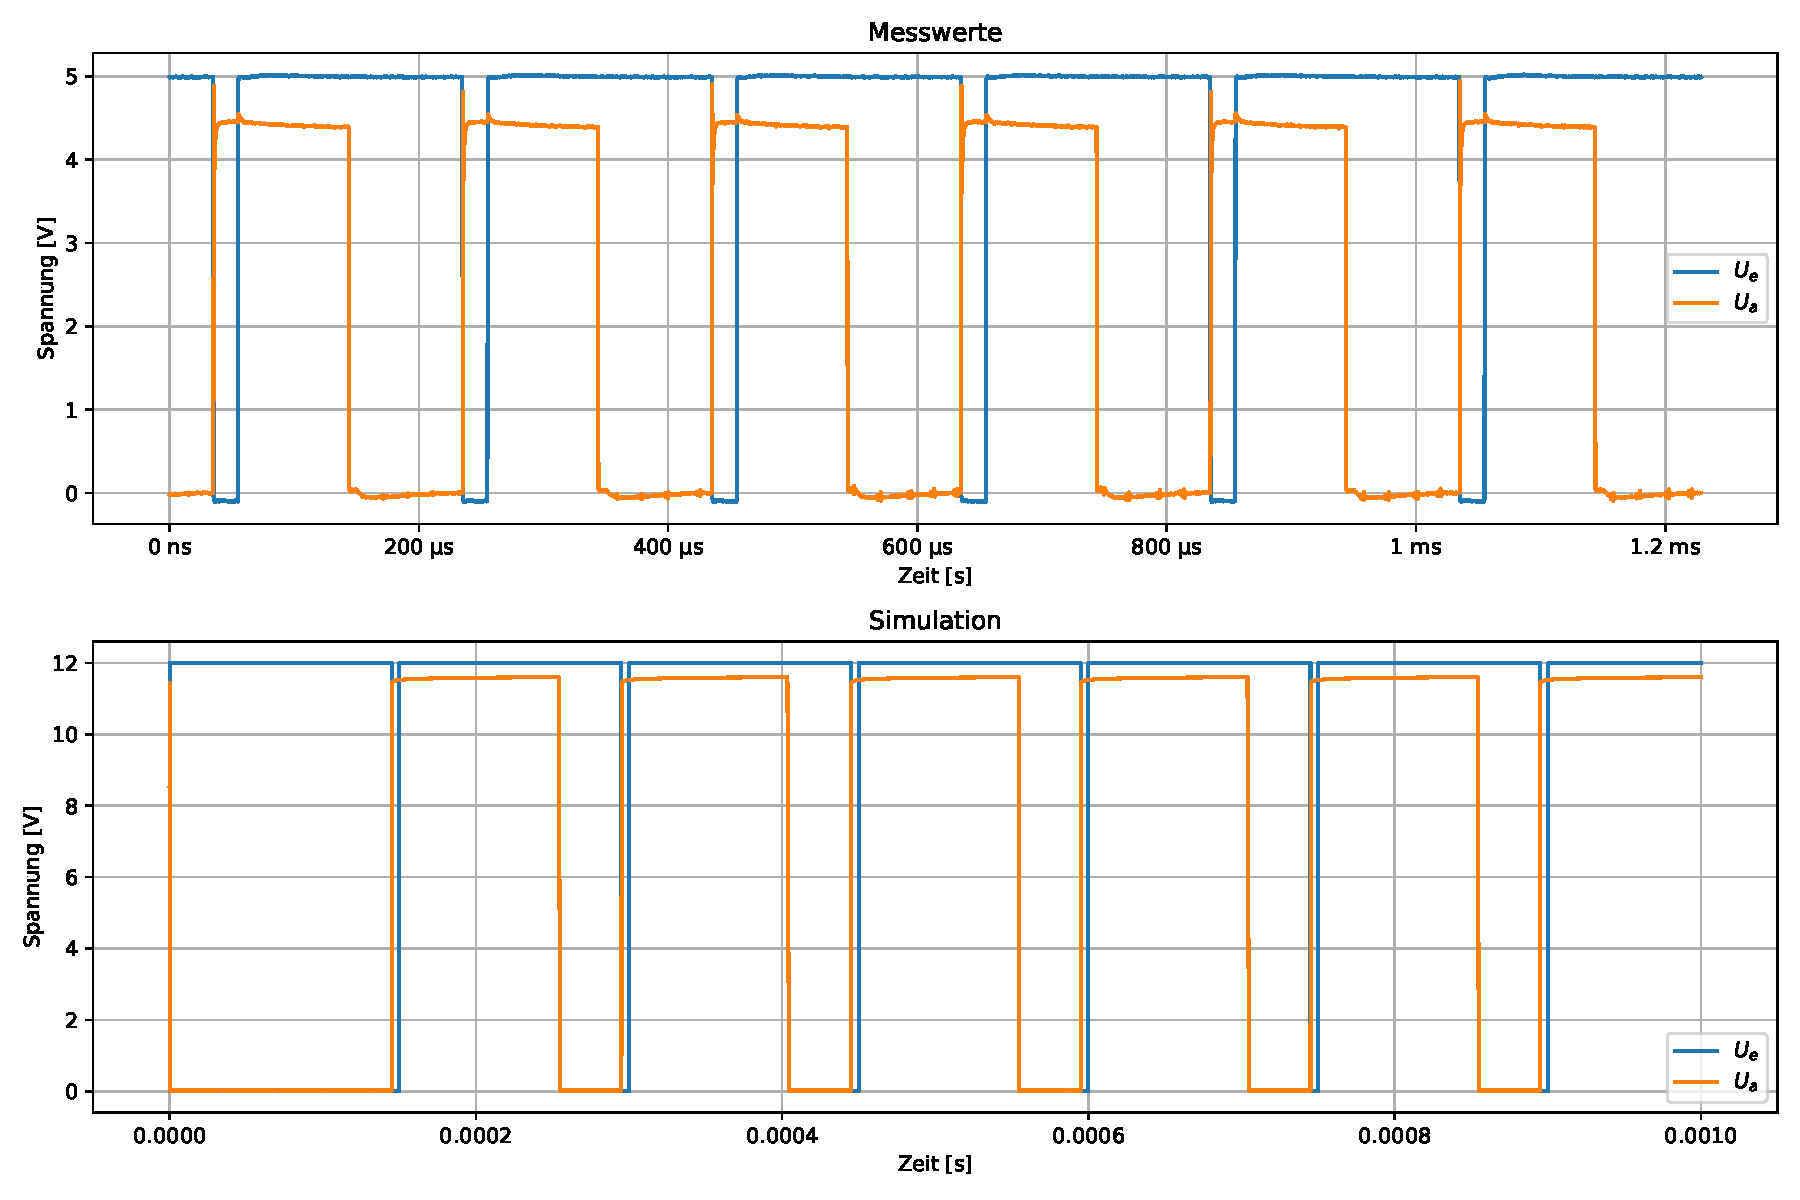
\includegraphics[width=\linewidth]{Elektronik-Laborprotokoll_Filter/Plots/monoflop.pdf}
  \caption{Monoflop-Diagram}
  \label{fig:monoflop}
\end{figure}

In Abbildung \ref{fig:monoflop} befindet sich der NE555 im monostabilen Modus, auch als Monoflop bezeichnet. Ein sehr kurzer Impuls, der eine konstante Spannung für eine über einen einstellbaren Widerstand festgelegte Zeit erzeugt, wird als Eingangsimpuls verwendet. Die resultierende Grafik zeigt einen klaren Anstieg des Ausgangssignals auf HIGH nach dem Triggerimpuls, gefolgt von einem Abfall auf LOW nach Ablauf der eingestellten Zeit. Aufgrund der Einschränkungen bei den Waveforms wird die VCC-Spannung hier mit \SI{5}{\volt} angelegt, während bei den anderen NE555-Schaltungen eine Versorgung von \SI{12}{\volt} verwendet wurde.

Die Zeitkonstante, die aus den Messdaten ermittelt wurde, beträgt ungefähr \SI{88,55}{\micro\second}. Die Abweichung von dem Zielwert \SI{100}{\micro\second} ist auf die nicht idealen Bauteilen und Messungen zurückzuführen.

\subsection{Dreieck-Rechteck-Oszillator}
%
Das Ziel des letzten Teilversuchs war, einen Dreieck-Rechteck-Oszillator aufzubauen. Dafür wird der Ausgang eines nichtinvertierenden Schmitt-Triggers an den Eingang eines invertierenden Integrator angeschlossen. Ebenfalls wird der Ausgang des invertierenden Integrator mit dem Eingang des nichtinvertierenden Schmitt-Triggers  verbunden.

Gegeben sind die Versorgungsspannung \( V_{CC} \) und die Schaltschwellen eines nicht-invertierenden Schmitt-Triggers \( V_{T+} = \frac{V_{CC}}{2} \) und \( V_{T-} = -\frac{V_{CC}}{2} \). Die Widerstände \( R_1 \) und \( R_2 \) sollen bestimmt werden. Die Beziehungen zwischen den Schaltschwellen und den Widerständen sind:

\begin{align}
    \frac{V_{T+}}{R_1} &= \frac{V_{CC} - (-V_{CC})}{R_2} \\
    \frac{V_{T-}}{R_1} &= \frac{-V_{CC} - (-V_{CC})}{R_2}
\end{align}

Die gegebenen Werte für \( V_{T+} \) und \( V_{T-} \) eingesetzt:

\begin{align}
    \frac{\frac{V_{CC}}{2}}{R_1} &= \frac{V_{CC}}{R_2} \\
    \frac{-\frac{V_{CC}}{2}}{R_1} &= \frac{-V_{CC}}{R_2}
\end{align}

Durch Kürzen von \( V_{CC} \) in beiden Gleichungen folgt:

\begin{align}
    \frac{1}{2R_1} &= \frac{1}{R_2} \\
    -\frac{1}{2R_1} &= -\frac{1}{R_2}
\end{align}

Beide Gleichungen führen zu demselben Ergebnis:

\begin{align}
    R_1 &= 2R_2
\end{align}

Die Widerstände des Schmitt-Triggers müssen mit einem Verhältnis von 1 zu 2 dimensioniert werden. Unter Berücksichtigung des Toleranzbereichs der Widerstandswerten wurden die Widerstände im Labor wie folgt dimensioniert: $R_1=\SI{22}{\kilo\ohm}$ und  $R_2=\SI{10}{\kilo\ohm}$.

Als zweites war das Ziel, einen Integrator mit einer sinnvoll gewählten Zeitkonstante zu dimensionieren.

Bei dem Integrator wird der Eingangstrom integriert.
Es gilt:
\begin{equation}
\label{eq:Integrator_I_E}
    I_E=\frac{U_E}{R_E}=\frac{V_{CC}}{R_E}
\end{equation}
Für die Berechnung der Kapazität eines Kondensators gilt:

\begin{equation}
    C= \frac{Q}{U}
\end{equation}

Durch die Gleichungen $Q=I_E t$ und $U=U_{ST,ON}-U_{ST,OFF}$ folgt:
\begin{align}
\label{eq:Gleichung_C}
     C= \frac{I_E\cdot t}{U_{ST,ON}-U_{ST,OFF}}
\end{align}
Wenn man die Gleichung \ref{eq:Integrator_I_E} in die Gleichung \ref{eq:Gleichung_C} einsetzt, gilt:
%
\begin{align*}
     R=\frac{V_{CC}\cdot t}{C\cdot(U_{ST,ON}-U_{ST,OFF})}
\end{align*}
Da der Tastgrad gleich \SI{50}{\percent} ist, gilt $t=\frac{T}{2}$. Daraus folgt:
\begin{align*}
     R= \frac{V_{CC}\cdot T}{2C\cdot(U_{ST,ON}-U_{ST,OFF})}
\end{align*}
Durch die Gleichung $f=\frac{1}{T}$ folgt:
\begin{align*}
     R=\frac{V_{CC}}{2fC\cdot(U_{ST,ON}-U_{ST,OFF})}
\end{align*}
Da 
die Schaltschwellen des Schmitt-Triggers bei $\frac{V_{CC}}{2}$ sind, gilt:
\begin{align*}
     R= \frac{V_{CC}}{2fC\cdot V_{CC}} =\frac{1}{2fC}
\end{align*}
Durch die Einsetzung der gegebenen Werte($f=\SI{2}{\kilo\hertz}$ und $C=\SI{100}{\nano\farad}$) gilt:
\begin{align*}
     R =\frac{1}{2\cdot\SI{2}{\kilo\hertz}\cdot\SI{100}{\nano\farad}}=\SI{2,5}{\kilo\ohm}
\end{align*}
Das heißt, dass der Widerstand des Integrators einen Wert von \SI{2,5}{\kilo\ohm} betragen soll.\\
%
In der Abbildung \ref{fig:dreieckoszillator} ist das Dreieck-Rechteck-Oszillator dargestellt.
%
\begin{figure}[H]
  \centering
  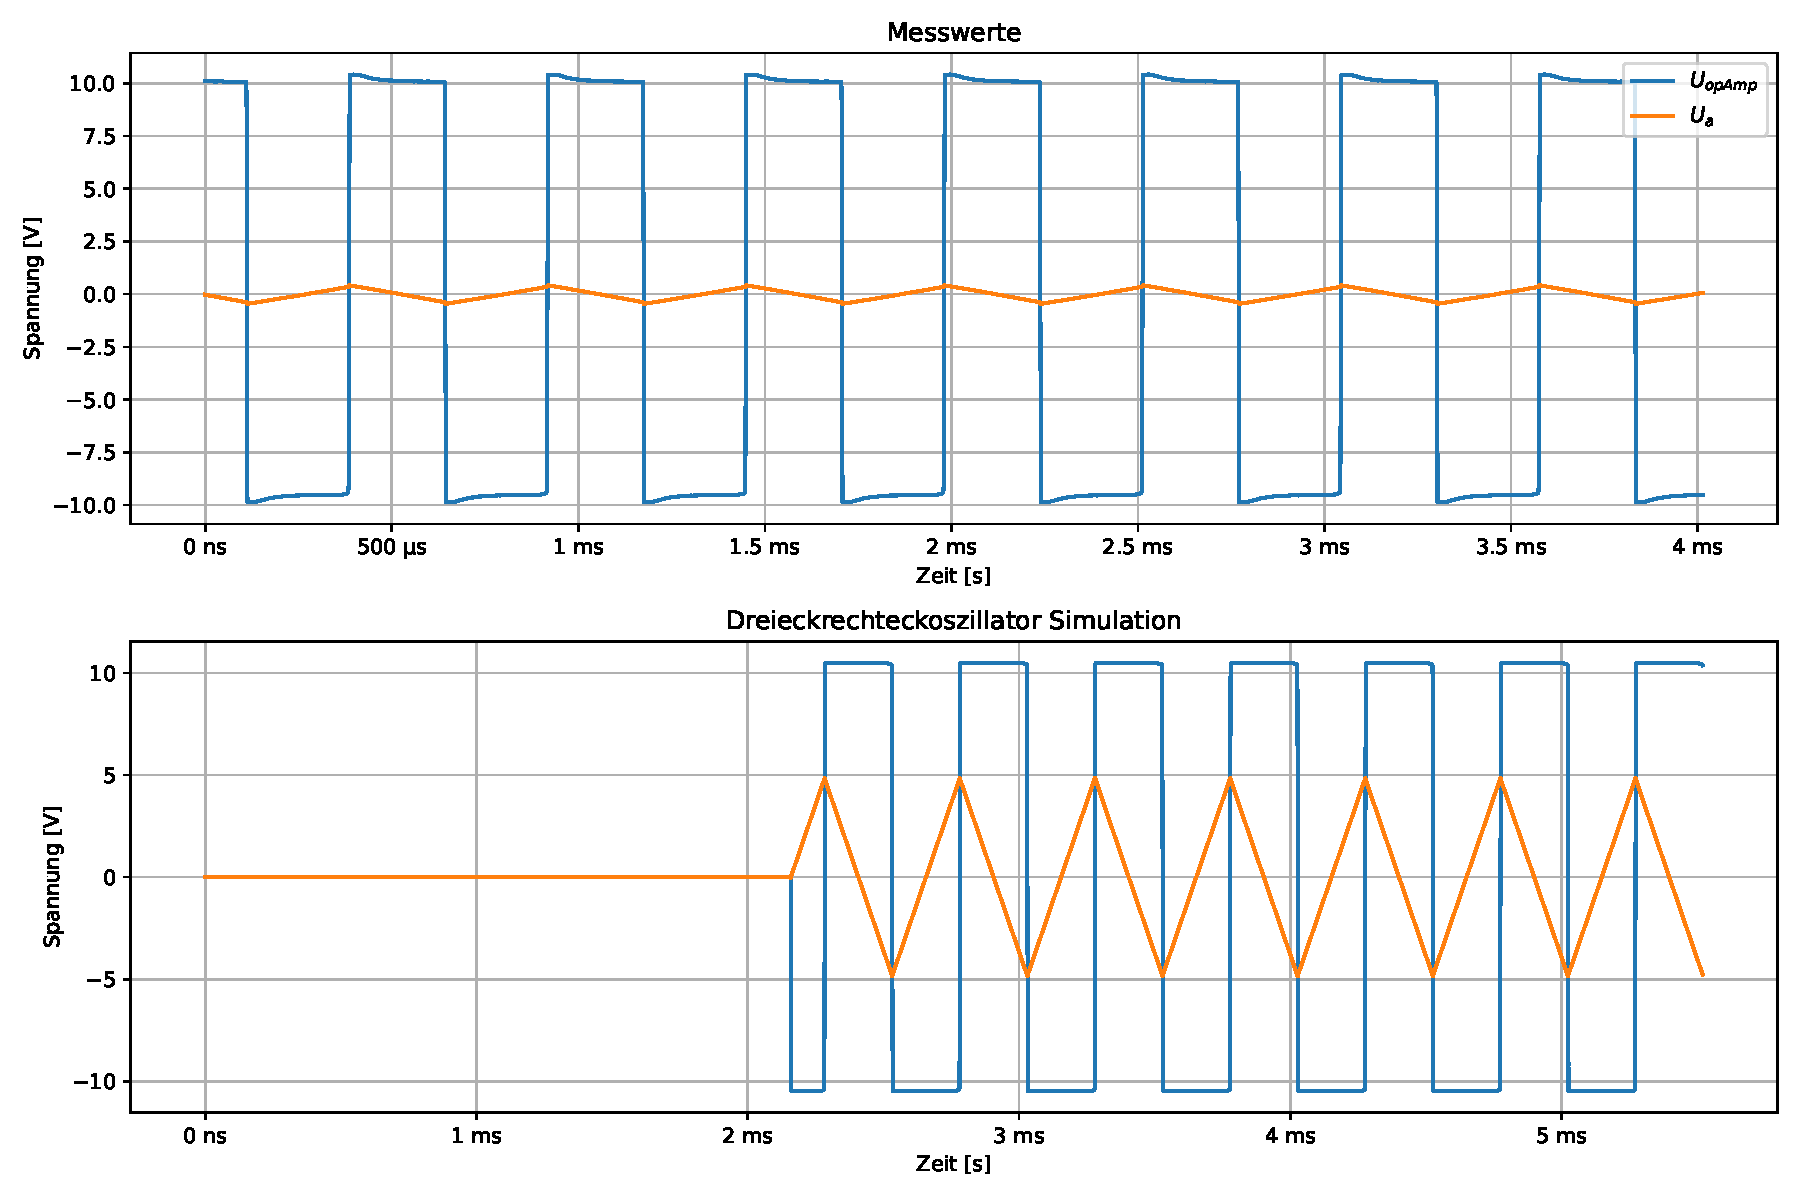
\includegraphics[width=\linewidth]{Elektronik-Laborprotokoll_Filter/Plots/dreieckoszillator.pdf}
  \caption{Dreieck-Rechteck-Oszillator Diagramm}
  \label{fig:dreieckoszillator}
\end{figure}

Auf dem Diagramm wird deutliche Abweichungen von der Simulation beobachtet. 
Es ist ersichtlich, dass die Oszillation eine gewisse Zeit benötigt, um sich zu ``aktivieren'', 
weshalb die Werte von \SI{0}{\milli\second} bis \SI{2}{\milli\second} nahezu Null sind. Ab \SI{2,2}{\milli\second} beginnt das Signal sichtbar zu werden. 
In der Simulation variiert das Dreiecksignal zwischen -5V und 5V. Vergleichen wir die Plots, 
fällt auf, dass das gemessene Dreiecksignal eine geringere Amplitude aufweist. Mögliche Ursachen hierfür könnten 
eine fehlerhafte Messung oder signifikante Messabweichungen sein. In der Simulation lassen sich ähnliche Ergebnisse 
erzielen, wenn der \(2,7\, \text{k}\Omega\)-Widerstand mit dem \(10\, \text{k}\Omega\)-Widerstand vertauscht wird. 
 Es ist auch denkbar, dass die Simulation die Verluste des Kondensators nicht berücksichtigt, was eine exakte Nachbildung des Signals verhindert.
 

 Die Frequenz des oszillierten Signals nach den Messwerten stimmt schon gut mit der Sollwert $f=\SI{2}{\kilo\hertz}$ überein.





